


	
	
{\color{Blue}{\subsection{Overview}}}

From the client standpoint, there are two applications, each one characterized by a independent architecture. Both ones communicate with TrackMe servers using the client-server paradigm. 


{\color{Blue}{\subsection{Component View}}}
T
{\color{Blue}{\subsubsection{Client Side}}}
Starting from the interface to the external sensors, the main problem related to the app separation is due to the fact that if the applications are running at a certain moment both of them could theoretically access the same monitoring device, providing to the server an identical sample. As anticipated in the Overview part, both the applications at clien side implement a personal hardware interface to the connected monitoring devices. This decision seems to introduce redundancy in code since a simple third service running in background could manage the connected devices and dispatch data between the two applications, unfortunately communication among running processes follows strict rules in many mobile OSs, someone only allows message exchanging. This makes more difficult to implement a mechanism of access to the monitoring sensors involving at most three different processes. Furthermore, relying on an HW manager service exposes both the apps to possible internal DOS attacks, since another malicious app could flood of messages the background service preventing the main application to allocate accesses to connected sensors.

\begin{figure}[H]
	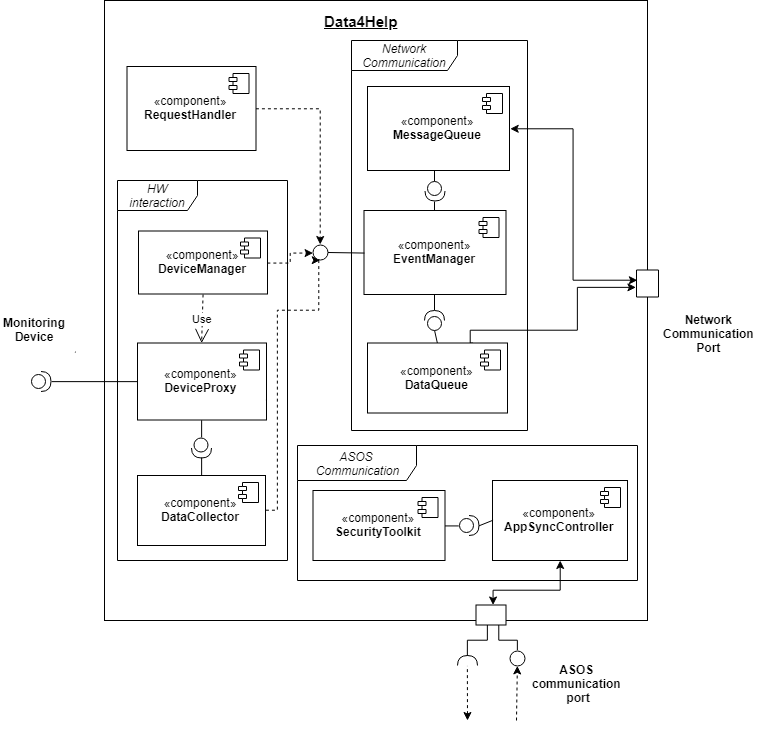
\includegraphics[scale=0.5]{images/uml/D4H_component}
\end{figure}

It has been decided to create a communication interface between D4H and ASOS, for synchronizing data collection and preventing both the applications to access the same information. This task should be protected in order to avoid other processes to send false messages to one of them. A security toolkit provides encryption mechanism to this end.
\begin{figure}[H]
	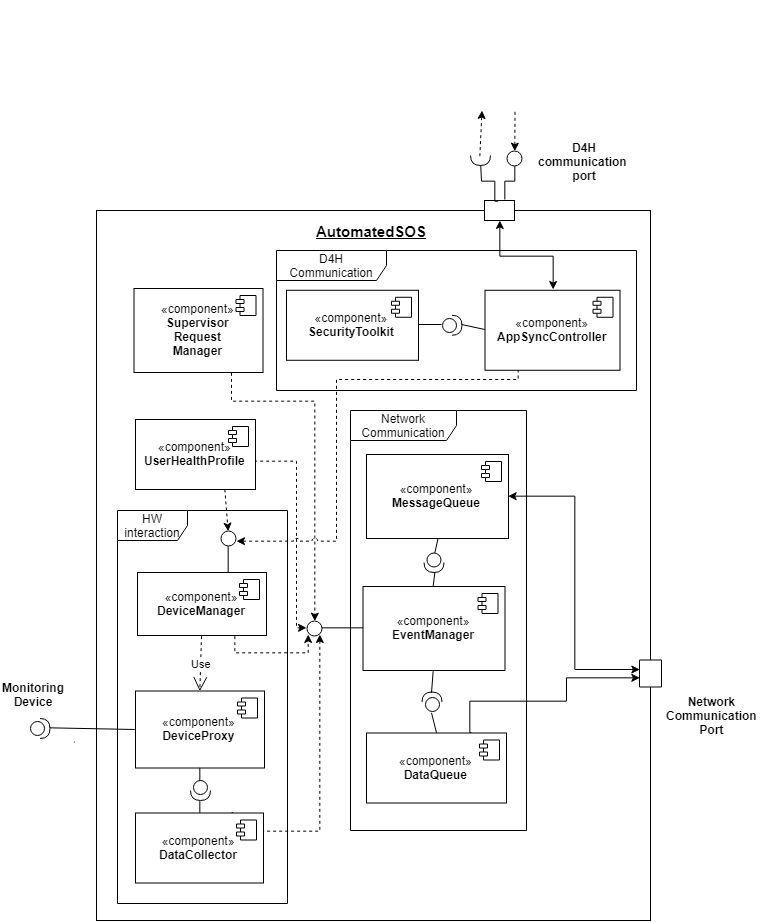
\includegraphics[scale=0.5]{images/uml/ASOS_component}
\end{figure}




{\color{Blue}{\subsection{Deployment View}}}


{\color{Blue}{\subsection{Runtime View}}}


{\color{Blue}{\subsection{Component Interfaces}}}


{\color{Blue}{\subsection{Selected Architectural Styles and Patterns}}}


{\color{Blue}{\subsection{Other Design Decisions}}}
	
